\documentclass{standalone}
\usepackage{tikz}

\begin{document}
	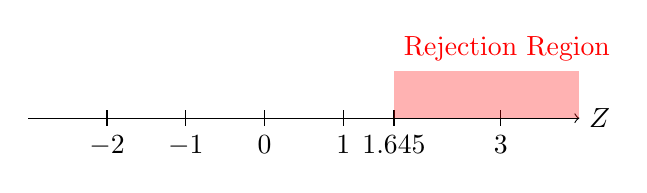
\begin{tikzpicture}
		% Draw x-axis
		\draw[->] (-3,0) -- (4,0) node[right] {$Z$};
		
		% Mark values on the x-axis
		\foreach \x in {-2,-1,0,1,3}
		\draw (\x,0.1) -- (\x,-0.1) node[below] {$\x$};
		
		% Mark 1.645 on the x-axis
		\draw (1.645,0.1) -- (1.645,-0.1) node[below] {1.645};
		
		% Draw shaded region beyond 1.645
		\fill[red, opacity=0.3] (1.645,0) rectangle (4,0.6);
		
		% Label for the shaded region
		\node[red, above right] at (1.645,0.6) {Rejection Region};
	\end{tikzpicture}
\end{document}